\documentclass[12pt]{article}
\usepackage{tikz}
\usepackage{amsmath}
\usepackage{amsthm}
\usepackage{geometry}
\usepackage{enumitem}
\usepackage{xcolor}
\usepackage{tcolorbox}
\usepackage{mdframed}
\usepackage{booktabs}
\usepackage{bm}
\usetikzlibrary{automata, positioning, arrows.meta, calc}

% Better page margins
\geometry{margin=1in}

% Custom colors
\definecolor{statecol}{RGB}{70,130,180}
\definecolor{transitioncol}{RGB}{0,100,0}

\begin{document}
	
	% Title page styling
	\title{\Large\textbf{CSL253 - Theory of Computation}\\[0.5em]
		\large Tutorial 2}
	\author{}
	\date{}
	\maketitle
	
	% Team members in a nice box
	\begin{tcolorbox}[
		title=\textbf{Team Members},
		colback=white,
		colframe=statecol,
		arc=0mm
		]
		\begin{enumerate}[leftmargin=*]
			\item Kartikeya Nainakhwal - 12341090
			\item Paritosh Lahre - 12341550
			\item Rahul Dev Reddy - 12342390
		\end{enumerate}
	\end{tcolorbox}
	
	% Question in a colored box
	\begin{tcolorbox}[
		title=\textbf{Question 2},
		colback=white,
		colframe=transitioncol,
		arc=0mm
		]
		Give state diagrams of NFAs with the specified number of states recognizing each of the following languages. In all parts the alphabet is \{0,1\}.
		\begin{enumerate}
			\item The language \{$\omega$ $|$ $\omega$ ends with 001 with three states\}\\
			\item The language \{$\omega$ $|$ $\omega$ contains the substring 0101, i.e., w = x0101y for some x and y\}  with five states\\
			\item The language \{$\omega$ $|$ $\omega$ contains an even number of 0s, or contains exactly two 1s\}  with six states\\ 
			\item The language \{0\} with two states\\
			\item The language 0*1*0+ with three states\\
			\item The language 1*(001+)* with three states\\
			\item The language \{e\} with one state\\
			\item The language 0* with one state
		\end{enumerate}
	\end{tcolorbox}
	
	\newpage
	\section*{Solution}
	
	\subsection*{1. \underline{Accepts strings ends with 001} } 
	\vspace{2mm}
	\subsubsection*{\underline{Language}}
	\begin{tcolorbox}[colback=white,colframe=transitioncol,arc=0mm]
		$A_1 =$ \{$\omega$ $|$ $\omega$ ends with 001 with three states\}
	\end{tcolorbox}
	
	\subsection*{\underline{Issue with the Problem Statement}}
	The problem statement requires constructing an NFA with only three states to recognize strings ending in "001." However, a three-state NFA cannot correctly enforce this condition. The minimal correct NFA for this language requires at least four states:
	
	\begin{itemize}
		\item One state for tracking the start.
		\item One state for detecting the first `0'.
		\item One state for detecting `00'.
		\item One state for accepting upon encountering `001'.
	\end{itemize}
	
	If we restrict the NFA to three states, it would either fail to distinguish between required patterns or accept incorrect strings, such as "01." Thus, the problem should either specify four states or redefine the accepted strings.
	
	\subsection*{\underline{Corrected NFA Diagram (Four States)}}
	\begin{center}
		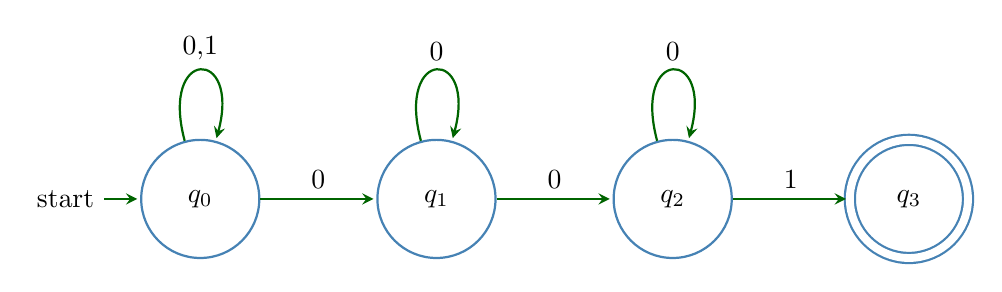
\begin{tikzpicture}[
			shorten >=1pt,
			node distance=3cm,
			on grid,
			auto,
			state/.style={
				draw=statecol,
				circle,
				minimum size=15mm,
				thick,
				fill=white
			},
			accepting/.style={
				double distance=1mm,
				fill=white
			},
			every edge/.style={
				draw=transitioncol,
				->,
				>=stealth,
				thick
			}
			]
			% States
			\node[state, initial] (q0) {$q_0$};
			\node[state] (q1) [right=of q0] {$q_1$};
			\node[state] (q2) [right=of q1] {$q_2$};
			\node[state, accepting] (q3) [right=of q2] {$q_3$};
			
			% Transitions
			\path[->]
			(q0) edge [loop above] node {0,1} ()
			edge node {0} (q1)
			(q1) edge node {0} (q2)
			edge [loop above] node {0} ()
			(q2) edge node {1} (q3)
			edge [loop above] node {0} ();   
		\end{tikzpicture}
	\end{center}
	
	\subsection*{\underline{Defining the NFA}}
	We define the NFA as a five-tuple \(M_1 = (Q_1, \Sigma, \delta_1, q_0, F_1)\) where:
	\begin{itemize}[leftmargin=*]
		\item \textbf{States:} \(Q_1 = \{q_0, q_1, q_2, q_3\}\), where:
		\begin{itemize}
			\item \(q_0\): Initial state
			\item \(q_1\): After first `0'
			\item \(q_2\): After `00'
			\item \(q_3\): Accepting state (after `001')
		\end{itemize}
		\item \textbf{Alphabet:} \(\Sigma = \{0, 1\}\)
		
		\item \textbf{Transition Function:} \(\delta_1: Q_1 \times \Sigma \to Q_1\)
		
		\begin{mdframed}[linewidth=1pt, leftmargin=3cm, rightmargin=3.2cm]
			\[\delta(\text{\textit{current state}}, \text{\textit{input}}) = \text{\textit{next state}}\]
		\end{mdframed}
		
		The transitions are defined as follows:
		\begin{align*}
			\delta_1(q_0, 0) &= q_0,q_1 \\
			\delta_1(q_0, 1) &= q_0 \\
			\delta_1(q_1, 0) &= q_1,q_2 \\
			\delta_1(q_2, 0) &= q_3 \\
			\delta_1(q_2, 1) &= q_3
		\end{align*}
		
		\item \textbf{Initial State:} \(q_0\)
		
		\item \textbf{Acceptance States:} \(F_1 = \{q_3\}\)
	\end{itemize}
	
	
	\subsection*{\underline{Transition Table}}
	\begin{center}
		\begin{tabular}{ccc}
			\toprule
			\textbf{Current State} & \textbf{Input `0'} & \textbf{Input `1'} \\
			\midrule
			$q_0$ & $q_0,q_1$ & $q_0$ \\
			$q_1$ & $q_1,q_2$ & $-$ \\
			$q_2$ & $q_2$ & $q_3$ \\
			\bottomrule
		\end{tabular}
	\end{center}
	
	\newpage
	\subsection*{2. \underline{Accepts strings which contains substring 0101 using five states}}
	\vspace{2mm}
	\subsubsection*{\underline{Language}}
	\begin{tcolorbox}[colback=white,colframe=transitioncol,arc=0mm]
		$A_2 =$ \{$\omega$ $|$ $\omega$ contains the substring 0101, i.e., w = x0101y for some x and y\}
	\end{tcolorbox}
	
	\subsubsection*{\underline{Explanation}}
	This NFA is designed to recognize binary strings that contain the substring `0101`. It consists of five states:
	
	\begin{itemize}
		\item The automaton starts at $q_0$ and moves through states $q_1$, $q_2$, $q_3$, and finally $q_4$ as it reads the pattern `0101`.
		\item If the pattern `0101` appears anywhere in the input, the automaton reaches the accepting state $q_4$.
		\item Once in $q_4$, the automaton remains there for all further inputs, ensuring acceptance.
		\item Any other sequence of `0`s and `1`s keeps the automaton in its non-accepting states.
	\end{itemize}
	This automaton effectively captures the required substring using only five states, demonstrating an efficient finite state approach.
	\subsubsection*{\underline{NFA Diagram}}
	\begin{center}
		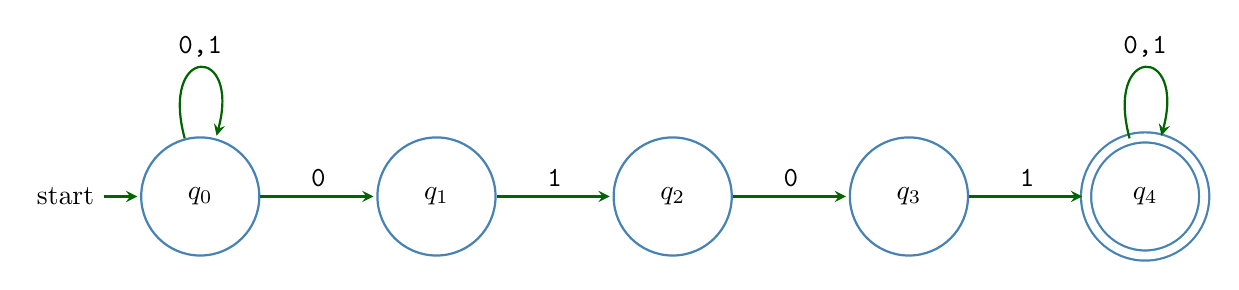
\begin{tikzpicture}[
			shorten >=1pt,
			node distance=3cm,
			on grid,
			auto,
			state/.style={
				draw=statecol,
				circle,
				minimum size=15mm,
				thick,
				fill=white
			},
			accepting/.style={
				double distance=1mm,
				fill=white
			},
			every edge/.style={
				draw=transitioncol,
				->,
				>=stealth,
				thick
			}
			]
			 % States
			\node[state, initial] (q0) {$q_0$};
			\node[state] (q1) [right=of q0] {$q_1$};
			\node[state] (q2) [right=of q1] {$q_2$};
			\node[state] (q3) [right=of q2] {$q_3$};
			\node[state, accepting] (q4) [right=of q3] {$q_4$};
			
			% Transitions
			\path[->]
			(q0) edge node {\texttt{0}} (q1)
			(q1) edge node {\texttt{1}} (q2)
			(q2) edge node {\texttt{0}} (q3)
			(q3) edge node {\texttt{1}} (q4)
			(q0) edge [loop above] node {\texttt{0,1}} ()
			(q4) edge [loop above] node {\texttt{0,1}} ();
		\end{tikzpicture}
	\end{center}
	
	\subsubsection*{\underline{Defining the NFA}}
	We define the NFA as a five-tuple $M_1 = (Q_1, \Sigma, \delta_1, q_0, F_1)$ where:
	
	\begin{itemize}
		\item \textbf{States:} $Q_1 = \{q_0, q_1, q_2, q_3, q_4\}$, where:
		\begin{itemize}
			\item $q_0$: Initial state
			\item $q_1$: Recognizing `0'
			\item $q_2$: Recognizing `01'
			\item $q_3$: Recognizing `010'
			\item $q_4$: Recognizing `0101' (accepting state)
		\end{itemize}
		\item \textbf{Alphabet:} $\Sigma = \{0, 1\}$
		\item \textbf{Transition Function:} $\delta_1: Q_1 \times \Sigma \to Q_1$
	\end{itemize}
	
	\begin{mdframed}[linewidth=1pt, leftmargin=3cm, rightmargin=3.2cm]
		\[\delta(\text{current state}, \text{input}) = \text{next state}\]
	\end{mdframed}
	
	The transitions are defined as follows:
	\begin{align*}
		\delta_1(q_0, 0) &= q_1 \\
		\delta_1(q_0, 1) &= q_0 \\
		\delta_1(q_1, 1) &= q_2 \\
		\delta_1(q_2, 0) &= q_3 \\
		\delta_1(q_3, 1) &= q_4 \\
		\delta_1(q_4, 0) &= q_4 \\
		\delta_1(q_4, 1) &= q_4
	\end{align*}
	
	\subsubsection*{\underline{Transition Table}}
	\begin{center}
		\begin{tabular}{ccc}
			\toprule
			\textbf{Current State} & \textbf{Input `0'} & \textbf{Input `1'} \\
			\midrule
			$q_0$ & $q_1$ & $q_0$ \\
			$q_1$ & - & $q_2$ \\
			$q_2$ & $q_3$ & - \\
			$q_3$ & - & $q_4$ \\
			$q_4$ & $q_4$ & $q_4$ \\
			\bottomrule
		\end{tabular}
	\end{center}
	
	
	\newpage
	\subsection*{3. \underline{Accepts strings which contains an even number of 0s or exactly two 1s} }
	\vspace{2mm}
	\subsubsection*{\underline{Language}}
	\begin{tcolorbox}[colback=white,colframe=transitioncol,arc=0mm]
		$A_1 =$ \{$\omega$ $|$ $\omega$ contains an even number of 0s, or contains exactly two 1s\}
	\end{tcolorbox}
	
	\subsubsection*{\underline{Explanation}}
	The given problem requires constructing an NFA that accepts strings satisfying one of the two conditions:
	\begin{itemize}
		\item The string contains an even number of 0s.
		\item The string contains exactly two 1s.
	\end{itemize}
	
	To solve this, we break the problem into two individual NFAs:
	\begin{enumerate}
		\item An NFA that accepts strings with an even number of 0s.
		\item An NFA that accepts strings containing exactly two 1s.
	\end{enumerate}
	
	Finally, we construct the union of these two NFAs using epsilon transitions, forming a new NFA that accepts a string if it satisfies either of the two conditions.
	
	\subsubsection*{\underline{Even Number of 0s}}
	This NFA maintains a state to track the parity of the number of 0s seen so far:
	\begin{itemize}
		\item The initial state is accepting, as a string with zero 0s is valid.
		\item Each occurrence of a 0 toggles the state between even and odd.
		\item The NFA remains in its current state when encountering a 1.
	\end{itemize}
	
	\subsubsection*{\underline{Exactly Two 1s}}
	This NFA tracks the number of 1s in the input:
	\begin{itemize}
		\item It starts in an initial state that transitions upon encountering a 1.
		\item After two 1s are received, the NFA moves to an accepting state.
		\item Any additional 1s push the NFA into a dead state.
		\item The NFA remains in its current state for 0s.
	\end{itemize}
	
	\subsubsection*{\underline{Union of the Two NFAs}}
	To combine the two NFAs into a single NFA, we introduce a new initial state with epsilon transitions to the start states of both NFAs. This allows the new NFA to nondeterministically choose which condition to track for any given input string. The final NFA correctly recognizes any string that meets either of the conditions.
	
	\subsubsection*{\underline{NFA Diagram}}
	\begin{center}
		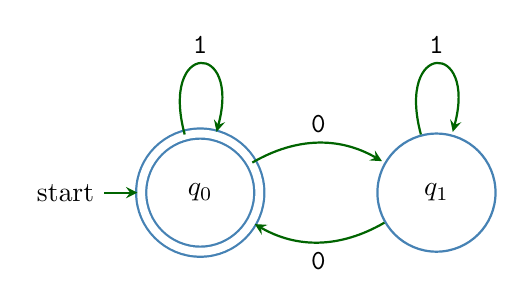
\begin{tikzpicture}[
			shorten >=1pt,
			node distance=3cm,
			on grid,
			auto,
			state/.style={
				draw=statecol,
				circle,
				minimum size=15mm,
				thick,
				fill=white
			},
			accepting/.style={
				double distance=1mm,
				fill=white
			},
			every edge/.style={
				draw=transitioncol,
				->,
				>=stealth,
				thick
			}
			]
			% States
			\node[state, initial, accepting] (q0) {$q_0$};
			\node[state] (q1) [right=of q0] {$q_1$};			
			% Transitions
			\path[->]
			(q0) edge [bend left] node {\texttt{0}} (q1)
			(q0) edge [loop above] node {\texttt1} ()
			(q1) edge [loop above] node {\texttt1} ()
			(q1) edge [bend left] node {\texttt{0}} (q0);
		\end{tikzpicture}
		
		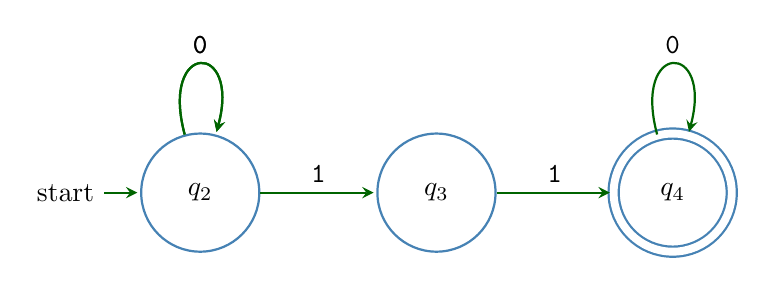
\begin{tikzpicture}[
			shorten >=1pt,
			node distance=3cm,
			on grid,
			auto,
			state/.style={
				draw=statecol,
				circle,
				minimum size=15mm,
				thick,
				fill=white
			},
			accepting/.style={
				double distance=1mm,
				fill=white
			},
			every edge/.style={
				draw=transitioncol,
				->,
				>=stealth,
				thick
			}
			]
			% States
			\node[state, initial] (q2) {$q_2$};
			\node[state] (q3)[right=of q2] {$q_3$};
			\node[state, accepting] (q4) [right=of q3] {$q_4$};
			
			% Transitions
			\path[->]
			(q2) edge node {\texttt{1}} (q3)
			(q3) edge node {\texttt{1}} (q4)
			(q2) edge [loop above] node {\texttt{0}} ()
			(q2) edge [loop above] node {\texttt{0}} ()
			(q4) edge [loop above] node {\texttt{0}} ();
		\end{tikzpicture}
		
		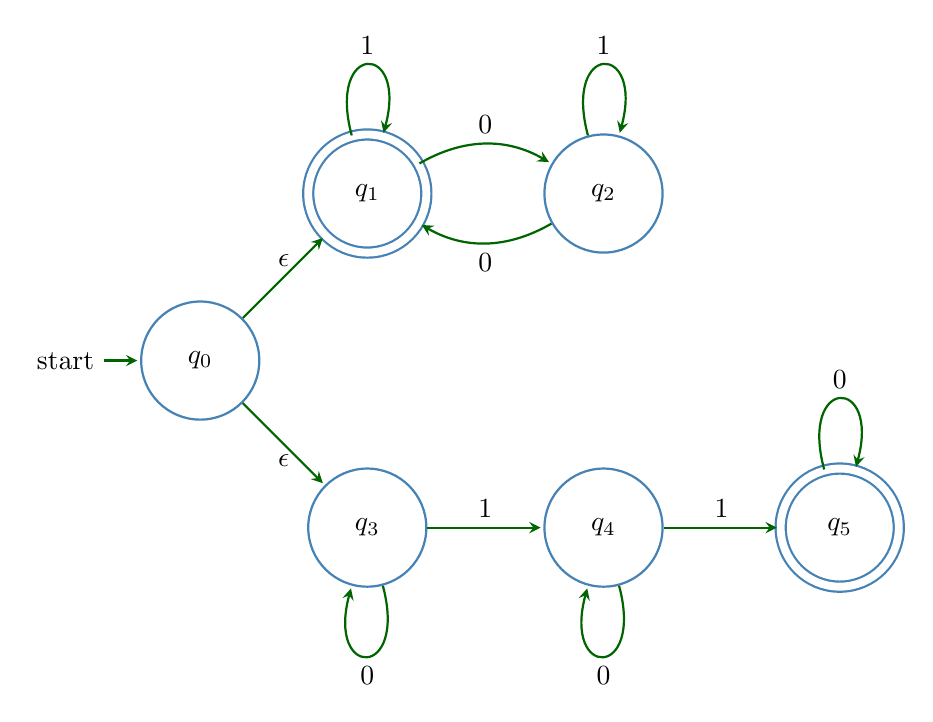
\begin{tikzpicture}[
			shorten >=1pt,
			node distance=3cm,
			on grid,
			auto,
			state/.style={
				draw=statecol,
				circle,
				minimum size=15mm,
				thick,
				fill=white
			},
			accepting/.style={
				double distance=1mm,
				fill=white
			},
			every edge/.style={
				draw=transitioncol,
				->,
				>=stealth,
				thick
			}
			]
			% States
			\node[state, initial] (q0)   {$q_0$}; 
			\node[state, accepting] (q1) [above right=of q0] {$q_1$}; 
			\node[state] (q2) [right=of q1] {$q_2$}; 
			\node[state] (q3) [below right=of q0] {$q_3$}; 
			\node[state] (q4) [right=of q3] {$q_4$}; 
			\node[state, accepting] (q5) [right=of q4] {$q_5$};
			
			
			% Transitions
			\path[->]
			(q0) edge [above] node {$\epsilon$} (q1)
			edge [below] node {$\epsilon$} (q3)
			(q1) edge [loop above] node {$1$} (q1)
			edge [bend left, above] node {$0$} (q2)  
			(q2) edge [loop above] node {$1$} (q2)
			edge [bend left, below] node {$0$} (q1)  
			(q3) edge [loop below] node {$0$} (q3)
			edge [above] node {$1$} (q4)
			(q4) edge [loop below] node {$0$} (q4)
			edge [above] node {$1$} (q5)
			(q5) edge [loop above] node {$0$} (q5);
		\end{tikzpicture}
	\end{center}
	
	\subsubsection*{\underline{Defining the NFA}}
	We define the NFA as a five-tuple \(M_1 = (Q_1, \Sigma, \delta_1, q_0, F_1)\) where:
	\begin{itemize}[leftmargin=*]
		\item \textbf{States:} \(Q_1 = \{q_0, q_1, q_2, q_3, q_4, q_5\}\), where:
		\begin{itemize}
			\item \(q_0\): Initial state
			\item \(q_1\): `1' state
			\item \(q_2\): Intermediate state
			\item \(q_3\): `0' state
			\item \(q_4\): Intermediate state
			\item \(q_5\): Accepting state
		\end{itemize}
		\item \textbf{Alphabet:} \(\Sigma = \{0, 1\}\)
		\item \textbf{Transition Function:} \(\delta_1: Q_1 \times (\Sigma \cup \{\varepsilon\}) \to 2^{Q_1}\)
	\end{itemize}
	
	\begin{mdframed}[linewidth=1pt, leftmargin=3cm, rightmargin=3.2cm]
		\[\delta_1(\text{current state}, \text{input}) = \text{next state(s)}\]
	\end{mdframed}
	
	The transitions are defined as follows:
	\begin{align*}
		\delta_1(q_0, \varepsilon) &= \{q_1, q_3\} \\
		\delta_1(q_1, 0) &= \{q_2\} \\
		\delta_1(q_1, 1) &= \{q_1\} \\
		\delta_1(q_2, 0) &= \{q_1\} \\
		\delta_1(q_2, 1) &= \{q_2\} \\
		\delta_1(q_3, 0) &= \{q_3\} \\
		\delta_1(q_3, 1) &= \{q_4\} \\
		\delta_1(q_4, 0) &= \{q_4\} \\
		\delta_1(q_4, 1) &= \{q_5\} \\
		\delta_1(q_5, 0) &= \{q_5\} \\
		\delta_1(q_5, 1) &= \{q_5\}
	\end{align*}
	
	\subsubsection*{\underline{Transition Table}}
	\begin{center}
		\begin{tabular}{ccc}
			\toprule
			\textbf{Current State} & \textbf{Input `0'} & \textbf{Input `1'} \\
			\midrule
			$q_0$ & $q_1, q_3$ (\(\varepsilon\)-transition) & - \\
			$q_1$ & $q_2$ & $q_1$ \\
			$q_2$ & $q_1$ & $q_2$ \\
			$q_3$ & $q_3$ & $q_4$ \\
			$q_4$ & $q_4$ & $q_5$ \\
			$q_5$ & $q_5$ & $q_5$ \\
			\bottomrule
		\end{tabular}
	\end{center}
	
	\newpage
	\subsection*{4. \underline{Accepts string 0 only using two states} } 
	\vspace{2mm}
	\subsubsection*{\underline{Regular Language}}
	\begin{tcolorbox}[colback=white,colframe=transitioncol,arc=0mm]
		$A_1 =$ \{$\omega$ $|$ $\omega$ is a string which contain only 0\}
	\end{tcolorbox}
	
	\subsubsection*{\underline{Explanation}}
	This finite automaton is designed to accept only the string "0" and reject all other strings, including the empty string and any string containing "1". The automaton consists of two states:
	
	\begin{itemize}
		\item $q_0$: The initial state.
		\item $q_1$: The accepting state, reached only when the input is exactly "0".
	\end{itemize}
	
	If the automaton reads the input "0", it transitions from $q_0$ to $q_1$, which is an accepting state. Any other input (including "1" or multiple characters) is not handled by a transition, effectively rejecting them.
	\subsubsection*{\underline{NFA Diagram}}
	\begin{center}
		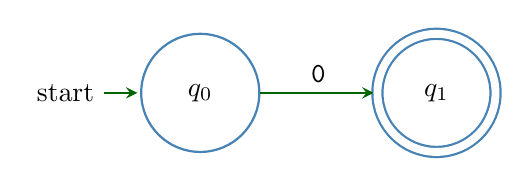
\begin{tikzpicture}[
			shorten >=1pt,
			node distance=3cm,
			on grid,
			auto,
			state/.style={
				draw=statecol,
				circle,
				minimum size=15mm,
				thick,
				fill=white
			},
			accepting/.style={
				double distance=1mm,
				fill=white
			},
			every edge/.style={
				draw=transitioncol,
				->,
				>=stealth,
				thick
			}
			]
			% States
			\node[state, initial] (q0) {$q_0$};
			\node[state, accepting] (q1) [right=of q0] {$q_1$};
			
			% Transitions
			\path[->]
			(q0) edge node {\texttt{0}} (q1);
		\end{tikzpicture}
	\end{center}
	
	\subsubsection*{\underline{Defining the NFA}}
	We define the NFA as a five-tuple \(M_1 = (Q_1, \Sigma, \delta_1, q_0, F_1)\) where:
	\begin{itemize}[leftmargin=*]
		\item \textbf{States:} \(Q_1 = \{q_0, q_1\}\), where:
		\begin{itemize}
			\item \(q_0\): Initial state
			\item \(q_1\): `0' state
		\end{itemize}
		\item \textbf{Alphabet:} \(\Sigma = \{0, 1\}\)
		
		\item \textbf{Transition Function:} \(\delta_1: Q_1 \times \Sigma \to Q_1\)
		
		\begin{mdframed}[linewidth=1pt, leftmargin=3cm, rightmargin=3.2cm]
			\[\delta(\text{\textit{current state}}, \text{\textit{input}}) = \text{\textit{next state}}\]
		\end{mdframed}
		
		The transitions are defined as follows:
		\begin{align*}
			\delta_1(q_0, 0) &= q_1 \\
		\end{align*}
		
		\item \textbf{Initial State:} \(q_0\)
		
		\item \textbf{Acceptance States:} \(F_1 = \{q_1\}\)
	\end{itemize}
	
	\subsubsection*{\underline{Transition Table}}
	\begin{center}
		\begin{tabular}{ccc}
			\toprule
			\textbf{Current State} & \textbf{Input `0'} & \textbf{Input `1'} \\
			\midrule
			$q_0$ & $q_1$ & - \\
			\bottomrule
		\end{tabular}
	\end{center}
	
	\newpage
	\subsection*{5. \underline{The language \( \{ 0^*1^* 0+\} \) with three states}}
	
	\vspace{2mm}
	
	\subsubsection*{\underline{Language}}
	\begin{tcolorbox}[colback=white,colframe=transitioncol,arc=0mm]
		\( A_1 =  0^*1^* 0+\) = This language consists of strings that start with any number of `0`s, followed by any number of `1`s, and end with at least one `0`.
	\end{tcolorbox}
	
	\subsubsection*{\underline{Explanation}}
	The given language consists of:
	\begin{itemize}
		\item Any number of `0`s at the beginning (including none at all).
		\item Followed by any number of `1`s (including none at all).
		\item Ending with at least one `0`, making it a necessary condition.
	\end{itemize}
	The purpose of this NFA is to efficiently recognize this pattern with a minimal number of states.
	
	\subsubsection*{\underline{NFA Diagram}}
	\begin{center}
		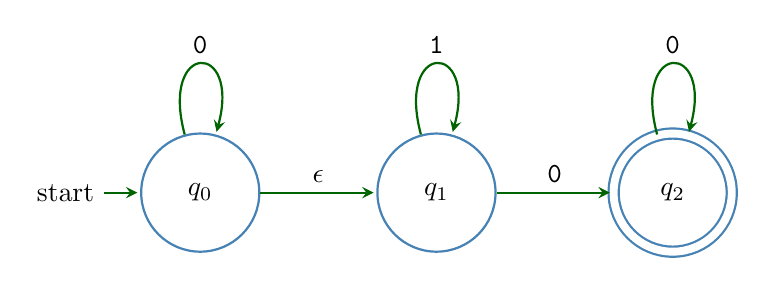
\begin{tikzpicture}[
			shorten >=1pt,
			node distance=3cm,
			on grid,
			auto,
			state/.style={
				draw=statecol,
				circle,
				minimum size=15mm,
				thick,
				fill=white
			},
			accepting/.style={
				double distance=1mm,
				fill=white
			},
			every edge/.style={
				draw=transitioncol,
				->,
				>=stealth,
				thick
			}
			]
			% States
			\node[state, initial] (q0) {$q_0$};
			\node[state] (q1) [right=of q0] {$q_1$};
			\node[state,accepting] (q2) [right=of q1] {$q_2$};
			
			% Transitions
			\path[->]
			(q0) edge [loop above] node {\texttt{0}} ()  % q0 loops on '0'
			edge node {\(\epsilon\)} (q1)  % q0 to q1 on '1'
			(q1) edge [loop above] node {\texttt{1}} ()  % q1 loops on '1'
			edge node {\texttt{0}} (q2)  % q1 to q2 on '0'
			(q2) edge [loop above] node {\texttt{0}} (); % q2 loops on '0'
		\end{tikzpicture}
	\end{center}
	
	\subsubsection*{\underline{Defining the NFA}}
	We define the NFA as a five-tuple \(M = (Q, \Sigma, \delta, q_0, F)\) where:
	
	\begin{itemize}[leftmargin=*]
		\item \textbf{States:} \(Q = \{q_0, q_1, q_2\}\), where:
		\begin{itemize}
			\item \(q_0\): Initial state (handles leading `0`s)
			\item \(q_1\): Intermediate state (handles `1`s)
			\item \(q_2\): Accepting state (ensures at least one 0 at the end)
		\end{itemize}
		
		\item \textbf{Alphabet:} \(\Sigma = \{0,1\}\)
		
		\item \textbf{Transition Function:} \(\delta: Q \times \Sigma \to Q\)
		
		\begin{mdframed}[linewidth=1pt, leftmargin=3cm, rightmargin=3.2cm]
			\[\delta(\text{\textit{current state}}, \text{\textit{input}}) = \text{\textit{next state}}\]
		\end{mdframed}
		
		The transitions are defined as follows:
		\begin{align*}
			\delta(q_0, 0) &= q_0 \\
			\delta(q_0, \epsilon) &= q_1 \\
			\delta(q_1, 1) &= q_1 \\
			\delta(q_1, 0) &= q_2 \\
			\delta(q_2, 0) &= q_2
		\end{align*}
		
		\item \textbf{Initial State:} \(q_0\)
		
		\item \textbf{Acceptance States:} \(F = \{q_2\}\)
	\end{itemize}
	
	\subsubsection*{\underline{Transition Table}}
	\begin{center}
		\begin{tabular}{ccc}
			\toprule
			\textbf{Current State} & \textbf{Input `0'} & \textbf{Input `1'} \\
			\midrule
			$q_0$ & $q_0$ & - \\
			$q_1$ & $q_2$ & $q_1$ \\
			$q_2$ & $q_2$ & - \\
			\bottomrule
		\end{tabular}
	\end{center}
	
	\newpage
	\subsection*{6. \underline{The language $1^*(001+)^*$ with three states} } 
	\vspace{2mm} 
	
	\subsubsection*{\underline{Regular Language}} 
	\begin{tcolorbox}[colback=white,colframe=transitioncol,arc=0mm] 
		\( A_1 = 1^*(001+)^*\) = The language consists of strings that may contain any number of 1`s followed by at least one occurrence of `001`, which can repeat any number of times.
	\end{tcolorbox} 
	\subsubsection*{\underline{Explanation}} 
	This NFA accepts strings that consist of any number of 1s followed by at least one occurrence of `001`, which can repeat. Here’s how it works:
	\begin{itemize} 
		\item The automaton starts in state $q_0$.
		\item While reading `1`, it remains in $q_0$.
		\item Upon encountering a `0`, it transitions to $q_1$.
		\item A second `0` moves it to $q_2$.
		\item A `1` from $q_2$ sends it back to $q_0$, completing one cycle of `001`.
		\item The accepting state is $q_0$, ensuring at least one full `001` pattern is read for a valid string.
	\end{itemize} 
	This minimal NFA with three states efficiently captures the essence of the given language.
	\subsubsection*{\underline{NFA Diagram}} 
	\begin{center} 
		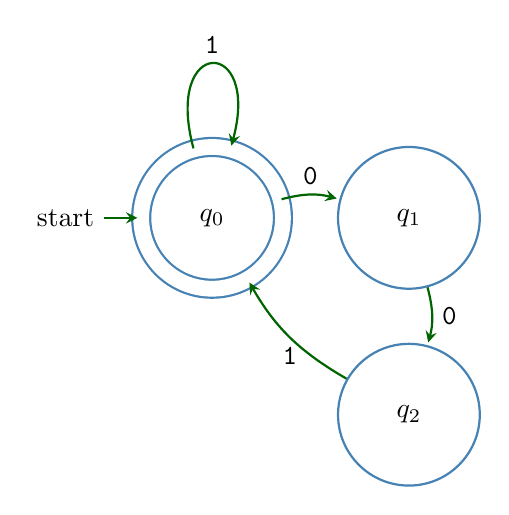
\begin{tikzpicture}[
			shorten >=1pt,
			node distance=2.5cm, 
			on grid,
			auto,
			state/.style={
				draw=statecol,
				circle,
				minimum size=18mm, 
				thick,
				fill=white
			},
			accepting/.style={
				double distance=2mm, 
				fill=white
			},
			every edge/.style={
				draw=transitioncol,
				->,
				>=stealth,
				thick
			}
			] 
			% States
			\node[state, initial, accepting] (q0) {$q_0$}; 
			\node[state] (q1) [right=of q0] {$q_1$}; 
			\node[state] (q2) [below=of q1] {$q_2$}; 
			
			% Transitions
			\path
			(q0) edge [loop above] node {\texttt{1}} () 
			edge [bend left=15] node [above] {\texttt{0}} (q1) 
			(q1) edge [bend left=15] node [right] {\texttt{0}} (q2) 
			(q2) edge [bend left=15] node [below] {\texttt{1}} (q0);
		\end{tikzpicture}
	\end{center} 
	
	\subsubsection*{\underline{Defining the NFA}} 
	We define the NFA as a five-tuple \(M = (Q, \Sigma, \delta, q_0, F)\) where: 
	
	\begin{itemize} 
		\item \textbf{States:} \(Q = \{q_0, q_1, q_2\}\)
		\begin{itemize} 
			\item \(q_0\): Initial and accepting state 
			\item \(q_1\): Intermediate state after reading 0
			\item \(q_2\): Intermediate state after reading 00
		\end{itemize} 
		\item \textbf{Alphabet:} \(\Sigma = \{0,1\}\) 
		\item \textbf{Transition Function:} \(\delta: Q \times \Sigma \to Q\)
		\begin{mdframed}[linewidth=1pt] 
			\[\delta(\text{\textit{current state}}, \text{\textit{input}}) = \text{\textit{next state}}\] 
		\end{mdframed} 
		The transitions are defined as follows: 
		\begin{align*} 
			\delta(q_0, 1) &= q_0 \\ 
			\delta(q_0, 0) &= q_1 \\ 
			\delta(q_1, 0) &= q_2 \\ 
			\delta(q_2, 1) &= q_0 
		\end{align*} 
		\item \textbf{Initial State:} \(q_0\) 
		\item \textbf{Acceptance States:} \(F = \{q_0\}\) 
	\end{itemize} 
	
	\subsubsection*{\underline{Transition Table}} 
	\begin{center} 
		\begin{tabular}{ccc} 
			\toprule 
			\textbf{Current State} & \textbf{Input `0'} & \textbf{Input `1'} \\ 
			\midrule 
			$q_0$ & $q_1$ & $q_0$ \\ 
			$q_1$ & $q_2$ & - \\ 
			$q_2$ & - & $q_0$ \\ 
			\bottomrule 
		\end{tabular} 
	\end{center} 
	 
	
	\newpage
	\subsection*{7. \underline{The language \{\(\epsilon\)\} with one state} } \vspace{2mm} 
	
	\subsubsection*{\underline{Regular Language}} 
	\begin{tcolorbox}[colback=white, colframe=black, arc=0mm]
		\( A_1 = \{ \epsilon \} \) --- This language consists of only the empty string \( \epsilon \), meaning it contains no actual symbols.
	\end{tcolorbox}
		\subsubsection*{\underline{Explanation}} 
	This NFA represents the language \(\{\epsilon\}\), which contains only the empty string. The automaton consists of a single state, \(q_0\), which serves as both the initial and accepting state. Since the language contains no actual symbols, the alphabet is empty \(\Sigma = \emptyset\), meaning there are no transitions. The automaton accepts the empty string by default because the initial state is also an accepting state. Any input other than the empty string is not part of this language, making this the simplest possible NFA.
	\subsubsection*{\underline{NFA Diagram}} 
	\begin{center} 
		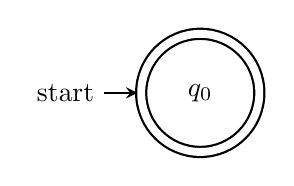
\begin{tikzpicture}[ 
			shorten >=1pt, 
			node distance=3cm, 
			on grid, 
			auto, 
			state/.style={ 
				draw=black, 
				circle, 
				minimum size=15mm, 
				thick, 
				fill=white 
			}, 
			accepting/.style={ 
				double distance=1mm, 
				fill=white 
			}, 
			every edge/.style={ 
				draw=black, 
				->, 
				>=stealth, 
				thick 
			} 
			] 
			% States 
			\node[state, initial, accepting] (q0) {$q_0$}; 
		\end{tikzpicture} 
	\end{center} 
	
	\subsubsection*{\underline{Defining the NFA}} 
	We define the NFA as a five-tuple \(M = (Q, \Sigma, \delta, q_0, F)\) where: 
	
	\begin{itemize}[leftmargin=*] 
		\item \textbf{States:} \(Q = \{q_0\}\), where:
		\begin{itemize} 
			\item \(q_0\): Initial and accepting state 
		\end{itemize} 
		\item \textbf{Alphabet:} \(\Sigma = \emptyset\) (since no input symbols are required)
		\item \textbf{Transition Function:} \(\delta: Q \times \Sigma \to Q\) (no transitions needed)
		\item \textbf{Initial State:} \(q_0\) 
		\item \textbf{Acceptance States:} \(F = \{q_0\}\) 
	\end{itemize} 
	
	\subsubsection*{\underline{Transition Table}} 
	\begin{center} 
		\begin{tabular}{c} 
			\toprule 
			\textbf{Current State} \\ 
			\midrule 
			$q_0$ (accepting) \\ 
			\bottomrule 
		\end{tabular} 
	\end{center} 
	
	
	
	\newpage
	\subsection*{8. \underline{ The language \(0^*\) with one state} } \vspace{2mm} 
	
	\subsubsection*{\underline{Regular Language}} 
	\begin{tcolorbox}[colback=white,colframe=transitioncol,arc=0mm] 
		$A_1 = 0^* =$ \{$\omega$ $|$ $\omega$ is language consists of all strings made up of zero or more occurrences of 0, including the empty string.\}\
	\end{tcolorbox} 
	
	\subsubsection*{\underline{Explanation}} 
	This NFA represents the language \(0^*\), which consists of any number of `0`s, including the empty string. The automaton has only one state, \(q_0\), which serves as both the initial and accepting state. The transition function ensures that any input `0` leads back to \(q_0\), allowing for repetition of `0`s indefinitely while remaining in an accepting state. Since the initial state is also an accepting state, the empty string is accepted by default.
	
	\subsubsection*{\underline{NFA Diagram}} 
	\begin{center} 
		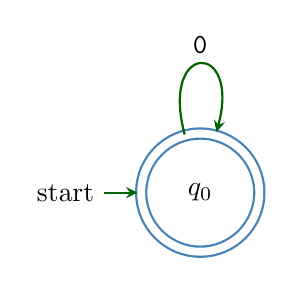
\begin{tikzpicture}[ 
			shorten >=1pt, 
			node distance=3cm, 
			on grid, 
			auto, 
			state/.style={ 
				draw=statecol, 
				circle, 
				minimum size=15mm, 
				thick, 
				fill=white 
			}, 
			accepting/.style={ 
				double distance=1mm, 
				fill=white 
			}, 
			every edge/.style={ 
				draw=transitioncol, 
				->, 
				>=stealth, 
				thick 
			} 
			] 
			% States 
			\node[state, initial, accepting] (q0) {$q_0$}; 
			
			% Transitions 
			\path[->] 
			(q0) edge [loop above] node {\texttt{0}} (); 
		\end{tikzpicture} 
	\end{center} 
	
	\subsubsection*{\underline{Defining the NFA}} 
	We define the NFA as a five-tuple \(M = (Q, \Sigma, \delta, q_0, F)\) where: 
	
	\begin{itemize}[leftmargin=*] 
		\item \textbf{States:} \(Q = \{q_0\}\), where:
		\begin{itemize} 
			\item \(q_0\): Initial and accepting state 
		\end{itemize} 
		\item \textbf{Alphabet:} \(\Sigma = \{0\}\) 
		\item \textbf{Transition Function:} \(\delta: Q \times \Sigma \to Q\) 
		\begin{mdframed}[linewidth=1pt, leftmargin=3cm, rightmargin=3.2cm] 
			\[\delta(q_0, 0) = q_0\] 
		\end{mdframed} 
		\item \textbf{Initial State:} \(q_0\) 
		\item \textbf{Acceptance States:} \(F = \{q_0\}\) 
	\end{itemize} 
	
	\subsubsection*{\underline{Transition Table}} 
	\begin{center} 
		\begin{tabular}{cc} 
			\toprule 
			\textbf{Current State} & \textbf{Input `0'} \\ 
			\midrule 
			$q_0$ & $q_0$ \\ 
			\bottomrule 
		\end{tabular} 
	\end{center} 
	
	\newpage
	\begin{tcolorbox}[
		title=\textbf{Question 4},
		colback=white,
		colframe=transitioncol,
		arc=0mm
		]
		Construct the state diagrams of NFAs recognizing the union of the languages described in:
		\begin{enumerate}
			\item[a.] $\{w \mid w \text{ contains the substring } 0101, \text{ i.e., } w = x0101y \text{ for some } x \text{ and } y\}$
			\item[b.] $\{w \mid w \text{ does not contain the substring } 1101\}$
		\end{enumerate}
	\end{tcolorbox}
	
	\section*{Solution}
	
	\subsection*{Step 1: Construct NFA for Language (a)}
	Language (a) is $\{w \mid w \text{ contains the substring } 0101\}$.
	
	\begin{itemize}
		\item \textbf{States}:
		\begin{itemize}
			\item $q_0$: Start state (no part of 0101 recognized yet).
			\item $q_1$: Recognized '0'.
			\item $q_2$: Recognized '01'.
			\item $q_3$: Recognized '010'.
			\item $q_4$: Recognized '0101' (accepting state).
		\end{itemize}
		
		\item \textbf{Transitions}:
		\begin{itemize}
			\item From $q_0$, on input '0', go to $q_0$,$q_1$.
			\item From $q_0$, on input '1', stay at $q_0$.
			\item From $q_1$, on input '1', go to $q_2$.
			\item From $q_2$, on input '0', go to $q_3$.
			\item From $q_3$, on input '1', go to $q_4$.
			\item From $q_4$, on any input, stay in $q_4$ (accepting state).
		\end{itemize}
		
		\item \textbf{Accepting State}: $q_4$.
	\end{itemize}
	
	\begin{center}
		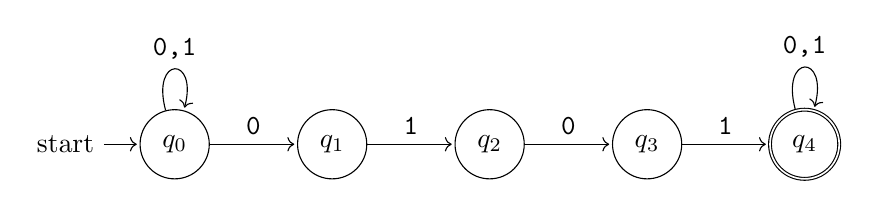
\begin{tikzpicture}[shorten >=1pt, node distance=2cm, on grid, auto]
			\node[state, initial] (q0) {$q_0$};
			\node[state] (q1) [right=of q0] {$q_1$};
			\node[state] (q2) [right=of q1] {$q_2$};
			\node[state] (q3) [right=of q2] {$q_3$};
			\node[state, accepting] (q4) [right=of q3] {$q_4$};
			
			\path[->]
			(q0) edge node {\texttt{0}} (q1)
			(q0) edge [loop above] node {\texttt{0,1}} ()
			(q1) edge node {\texttt{1}} (q2)
			(q2) edge node {\texttt{0}} (q3)
			(q3) edge node {\texttt{1}} (q4)
			(q4) edge [loop above] node {\texttt{0,1}} ();
			
		\end{tikzpicture}
	\end{center}
	
	\subsection*{Step 2: Construct NFA for Language (b)}
	Language (b) is $\{w \mid w \text{ does not contain the substring } 1101\}$.
	
	\begin{itemize}
		\item \textbf{States}:
		\begin{itemize}
			\item $p_0$: Start state (no part of 1101 recognized yet).
			\item $p_1$: Recognized '1'.
			\item $p_2$: Recognized '11'.
			\item $p_3$: Recognized '110'.
			\item $p_4$: Recognized '1101' (trap state, non-accepting).
		\end{itemize}
		
		\item \textbf{Transitions}:
		\begin{itemize}
			\item From $p_0$, on input '1', go to $p_0$,$p_1$.
			\item From $p_0$, on input '0', stay at $p_0$.
			\item From $p_1$, on input '1', go to $p_2$.
			\item From $p_1$, on input '0', return to $p_0$ (sequence broken).
			\item From $p_2$, on input '0', go to $p_3$.
			\item From $p_2$, on input '1', stay at $p_2$.
			\item From $p_3$, on input '1', go to $p_4$ (trap state).
			\item From $p_3$, on input '0', return to $p_0$ (sequence broken).
			\item From $p_4$, on any input, stay in $p_4$ (trap state).
		\end{itemize}
		
		\item \textbf{Accepting States}: All states except $p_4$.
	\end{itemize}
	
	\begin{center}
		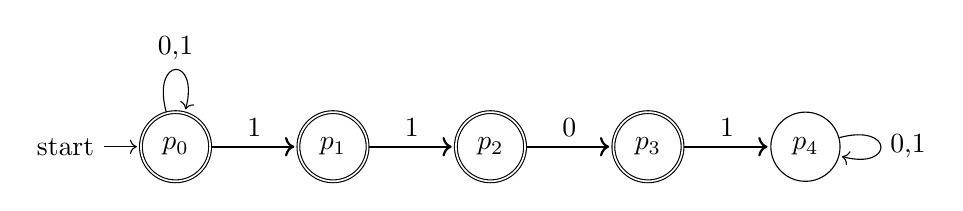
\begin{tikzpicture}[shorten >=1pt, node distance=2cm, on grid, auto]
			\node[state, initial,accepting] (p0) {$p_0$};
			\node[state, right of=p0,accepting] (p1) {$p_1$};
			\node[state, right of=p1,accepting] (p2) {$p_2$};
			\node[state, right of=p2,accepting] (p3) {$p_3$};
			\node[state, right of=p3] (p4) {$p_4$};
			
			\path[->]
			(p0) edge[loop above,auto] node{0,1} (0)
			(p0) edge[thick, auto] node{1} (p1)
			(p1) edge[thick, auto] node{1} (p2)
			(p2) edge[thick, auto] node{0} (p3)
			(p3) edge[thick, auto] node{1} (p4)
			(p4) edge[loop right, auto] node{0,1} (p4);
			
			
		\end{tikzpicture}
	\end{center}
	
	\subsection*{Step 3: Construct NFA for the Union of Languages (a) and (b)}
	To recognize the union of the two languages, we use the standard construction for the union of two NFAs.
	
	\begin{itemize}
		\item \textbf{New Start State}: Create a new start state $s_0$.
		
		\item \textbf{Transitions from $s_0$}:
		\begin{itemize}
			\item Add $\epsilon$-transitions from $s_0$ to the start states of the two NFAs ($q_0$ and $p_0$).
		\end{itemize}
		
		\item \textbf{States}: Combine the states of the two NFAs.
		
		\item \textbf{Transitions}: Keep all transitions from both NFAs.
		
		\item \textbf{Accepting States}: Any state that is an accepting state in either of the two NFAs is an accepting state in the new NFA.
	\end{itemize}
	
	\begin{center}
		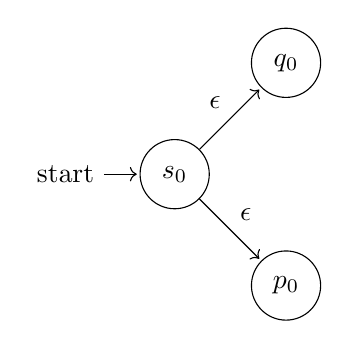
\begin{tikzpicture}[shorten >=1pt, node distance=2cm, on grid, auto]
			\node[state, initial] (s0) {$s_0$};
			\node[state, above right of=s0] (q0) {$q_0$};
			\node[state, below right of=s0] (p0) {$p_0$};
			
			\path[->]
			(s0) edge node {$\epsilon$} (q0)
			(s0) edge node {$\epsilon$} (p0);
		\end{tikzpicture}
	\end{center}
	
	\subsection*{Final NFA}
	The final NFA will have:
	\begin{itemize}
		\item A new start state $s_0$ with $\epsilon$-transitions to $q_0$ and $p_0$.
		\item All states and transitions from both NFAs.
		\item Accepting states are $q_4$ and all states from the second NFA except $p_4$.
	\end{itemize}
	
	This NFA will accept any string that is in language (a) or language (b).
	\newpage
	\begin{tcolorbox}[
		title=\textbf{Question 5},
		colback=white,
		colframe=transitioncol,
		arc=0mm
		]
		Prove that every NFA can be converted to an equivalent one that has a single accept state.
	\end{tcolorbox}
	\section{Introduction}
	A Nondeterministic Finite Automaton (NFA) is a theoretical computational model used in formal language theory. It is defined by a tuple $(Q, \Sigma, \delta, q_0, F)$ where:
	\begin{itemize}
		\item $Q$ is a finite set of states,
		\item $\Sigma$ is a finite set of input symbols (the alphabet),
		\item $\delta$ is the transition function: $\delta: Q \times \Sigma \to 2^Q$,
		\item $q_0 \in Q$ is the initial state, and
		\item $F \subseteq Q$ is the set of accept states.
	\end{itemize}
	An NFA accepts a string if there exists a sequence of transitions that lead to an accept state after consuming the entire input.
	
	\section{Conversion to an NFA with a Single Accept State}
	Given an NFA $(Q, \Sigma, \delta, q_0, F)$, we can construct an equivalent NFA $(Q_{\text{new}}, \Sigma, \delta_{\text{new}}, q_0, F_{\text{new}})$ with a single accept state as follows:
	
	\begin{enumerate}
		\item Introduce a new accept state $q_{\text{new}}$.
		\item Modify the transition function by adding an $\epsilon$-transition from each state in $F$ to $q_{\text{new}}$.
		\item Define the new accept state as $F_{\text{new}} = \{q_{\text{new}}\}$.
	\end{enumerate}
	
	\section{Example: NFA with Two Accepting States}
	Consider an NFA with two accept states, $q_2$ and $q_3$, which accepts strings ending in either 01 or 10:
	
	\begin{center}
		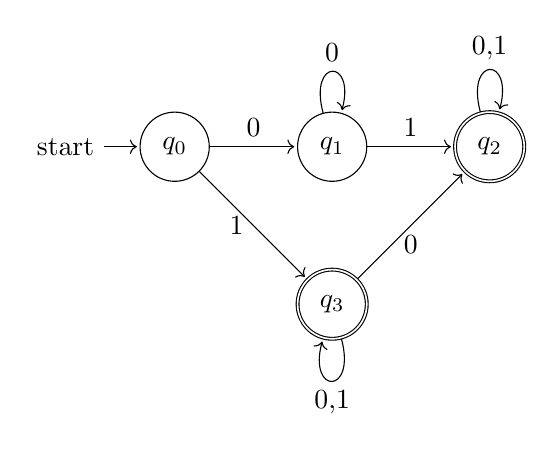
\begin{tikzpicture}[shorten >=1pt, node distance=2cm, on grid, auto]
			\node[state, initial] (q0) {$q_0$};
			\node[state] (q1) [right=of q0] {$q_1$};
			\node[state, accepting] (q2) [right=of q1] {$q_2$};
			\node[state, accepting] (q3) [below=of q1] {$q_3$};
			
			\path[->]
			(q0) edge [above] node {0} (q1)
			(q1) edge [above] node {1} (q2)
			(q0) edge [left] node {1} (q3)
			(q3) edge [below] node {0} (q2)
			(q1) edge [loop above] node {0} ()
			(q2) edge [loop above] node {0,1} ()
			(q3) edge [loop below] node {0,1} ();
		\end{tikzpicture}
	\end{center}
	
	Now, we convert this NFA to an equivalent one with a single accept state:
	
	\begin{center}
		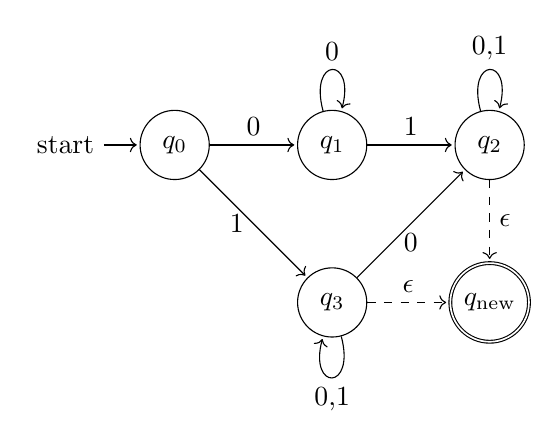
\begin{tikzpicture}[shorten >=1pt, node distance=2cm, on grid, auto]
			\node[state, initial] (q0) {$q_0$};
			\node[state] (q1) [right=of q0] {$q_1$};
			\node[state] (q2) [right=of q1] {$q_2$};
			\node[state] (q3) [below=of q1] {$q_3$};
			\node[state, accepting] (q_new) [below=of q2] {$q_{\text{new}}$};
			
			\path[->]
			(q0) edge [above] node {0} (q1)
			(q1) edge [above] node {1} (q2)
			(q0) edge [left] node {1} (q3)
			(q3) edge [below] node {0} (q2)
			(q1) edge [loop above] node {0} ()
			(q2) edge [loop above] node {0,1} ()
			(q3) edge [loop below] node {0,1} ()
			(q2) edge [dashed] node {$\epsilon$} (q_new)
			(q3) edge [dashed] node {$\epsilon$} (q_new);
		\end{tikzpicture}
	\end{center}
	
	\section{Proof of Equivalence}
	To show that both NFAs accept the same language:
	\begin{itemize}
		\item If the original NFA accepts a string, it must end in either $q_2$ or $q_3$. Since both states now have an $\epsilon$-transition to $q_{\text{new}}$, the new NFA will also accept the string.
		\item If the new NFA accepts a string, it must have reached state $q_{\text{new}}$, which can only occur through $q_2$ or $q_3$. Therefore, the original NFA must also have accepted the string.
	\end{itemize}
	Since both NFAs accept the same set of strings, they are equivalent.
	
	\section{Conclusion}
	We have successfully constructed an NFA with a single accept state that is equivalent to any given NFA, even one with multiple accept states. This proves that every NFA can be transformed into an equivalent one with exactly one accept state.
	
\end{document}